\chapter{Padrões de Projeto - \textit{Factory}, DAO e MVC}
\epigraph{``\textit{É longo o caminho que vai do projeto à coisa}''.}{Molière}

\lettrine[lines=4, lhang=0.1, lraise=0, loversize=0.2, findent=0.1em]{\textcolor{corAzulTema}{N}}{ESTE} Capítulo teremos como objetivo entender e aplicar os Padrões de Projeto \textit{Factory}, DAO e MVC. Além disso iremos aprender a integrar o acesso à banco de dados em uma aplicação Java.


\section{Introdução}

A partir de agora iremos dar um passo importantíssimo em nossos estudos sobre desenvolvimento de software, pois iremos aprender a lidar com um banco de dados em um sistema de testes que iremos construir. Isso nos dará o embasamento necessário para que no próximo Capítulo nós consigamos fazer essa mesma integração em aplicações Web. Além de aprendermos a conectar nossa aplicação com uma base de dados, iremos aprender também alguns padrões de projeto que nos ajudarão a organizar nossa aplicação de forma a melhorar sua manutenção. 

Antes de começarmos a discussão e a implementação desses padrões, nós precisamos preparar nosso ambiente de desenvolvimento. O NetBeans já temos instalado. O SGBD que iremos utilizar, o MariaDB\footnote{Provavelmente você deve ter instalado na sua máquina o MariaDB que é distribuído junto ao XAMPP}/MySQL, você provavelmente já deve ter instalado também. Com isso pronto, precisamos instalar uma ferramenta para nos ajudar a criar nossa base de dados. Iremos utilizar o MySQL Workbench, uma ferramenta gratuita para gerenciamento do MariaDB/MySQL. 


\section{Preparando o Ambiente}

Para começar, vamos fazer o download da ferramenta. Acesse o endereço \url{https://dev.mysql.com/downloads/workbench/}, escolha Microsoft Windows como plataforma, que provavelmente é o sistema operacional que você está utilizando e clique no botão ``\textit{Download}''. Fazendo isso, você será direcionado para uma página onde é requisitado um nome de usuário e senha. Se você não quiser se cadastrar (não precisa), clique no link embaixo do formulário de \textit{login} onde está escrito ``\textit{No thanks, just start my download}''. O download do instalador será iniciado.

Baixou? Legal! Execute o instalador. Na época da elaboração desse livro, a última versão disponível era a \texttt{8.0.25}. Basta seguir os passos, fazendo a instalação completa. Ao terminar, deixe marcada a opção \destaque{\textit{Launch MySQL Workbench now}} e clique em \destaque{\textit{Finish}}. Aguarde o MySQL Workbench abrir. A interface principal da versão 8.0.25 do Workbench pode ser vista na Figura~\ref{fig:cap04MySQLWorkbench}.

\FloatBarrier
\begin{figure}[!htbp]
    \centering
    \caption{Interface principal do MySQL Workbench}
    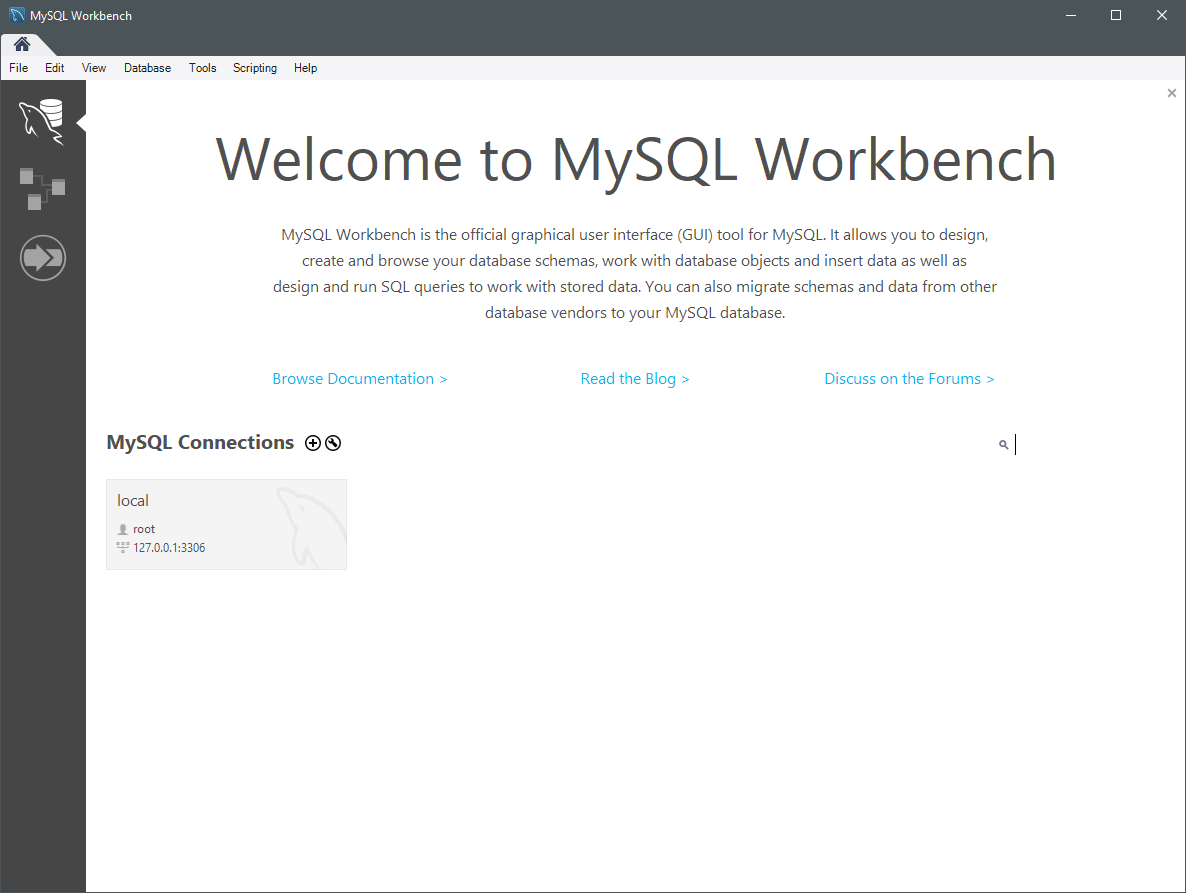
\includegraphics[scale=0.45]{imagens/cap04MySQLWorkbench}
    \\\textbf{Fonte:} Elaborada pelo autor
    \label{fig:cap04MySQLWorkbench}
\end{figure}
\FloatBarrier

Verifique se existe alguma instância configurada abaixo de \destaque{\textit{MySQL Connections}}, se não houver, clique em \destaque{\texttt{+}}. Um assistente aparecerá. Em \destaque{\textit{Connection Name:}} dê um nome para a conexão, pode ser qual você desejar. No meu caso, é ``localhost''. \destaque{\textit{Connection Method:}} deve ficar com a opção ``Standard (TCP/IP)'' selecionada. \destaque{\textit{Hostname:}} deve estar preenchido com o IP \texttt{127.0.0.1} que é o endereço de \textit{loopback}. Como o servidor está instalado na máquina que você está trabalhando, deixe como está. Em \destaque{\textit{Username:}} mantenha ``root'' e não será necessário configurar uma senha. Em \destaque{\textit{Port:}}, mantenha \texttt{3306}, que é a porta padrão que o MariaDB/MySQL ouve. Deixe \destaque{\textit{Default Schema:}} vazio. Note que estou assumindo que você está usando o MariaDB distribuído no XAMPP e que não realizou nenhuma mudança na instalação e no usuário administrador. Caso tenha realizado alguma alteração, você precisará replicá-las na configuração do MySQL Workbench. Clique no botão \destaque{\textit{Test Connection}}. A ferramenta vai avisar que há uma incompatibilidade de protocolos, pois ela está tentando conectar numa instância do MySQL, mas estamos rodando o MariaDB. Esse aviso pode ser ignorado, clicando em \destaque{\textit{Continue Anyway}}. Se tudo estiver correto, a conexão será bem sucedida, sendo avisada através de um diálogo com a mensagem ``\textit{Successfully made the MySQL connection}''. Lembre-se que o MariaDB/MySQL deve estar em execução! Por fim, clique no botão \destaque{\textit{OK}}, o diálogo será fechado e a conexão aparecerá.

Clique duas vezes na conexão criada. Novamente, será mostrado um aviso, dizendo sobre a incompatibilidade de protocolos. \textcolor{red}{\textbf{\underline{Não marque a opção} ``\textit{Don't show this message again}''}} e clique em \destaque{\textit{Continue Anyway}}. Pronto? Muito bem! Sempre que abrirmos o Workbench, essas configurações já estarão feitas, não se preocupe. Agora nós vamos criar uma base de dados para trabalharmos nos exemplos deste Capítulo.

Na interface que se abriu, do lado esquerdo, em \destaque{\textit{Navigator}} há duas abas que ficam abaixo. Uma é chamada \destaque{\textit{Administration}}, que é a que está selecionada por padrão, e outra chamada \destaque{\textit{Schemas}}. Clique em \destaque{\textit{Schemas}}. No aba de esquemas, na parte em branco, clique com o botão direito e escolha \destaque{\textit{Create Schema}}. Preencha o campo \destaque{\textit{Name:}} com ``testes\_padroes'' (sem as aspas) e deixe o campo \destaque{\textit{Charset/Collation:}} como ``Default Charset'' e ``Default Collation''. Clique em \destaque{\textit{Apply}}. Um diálogo será aberto para mostrar o código SQL que será executado. Clique em \destaque{\textit{Apply}} e se der tudo certo, clique em \destaque{\textit{Finish}}. A aba de criação de esquemas continuará aberta, podendo ser fechada. Ao terminar esse processo, o novo esquema (vamos chamar os esquemas de base de dados a partir de agora) será criado e estará listado na lista \destaque{\textit{SCHEMAS}}. Vamos configurar a base de dados que acabamos de criar como padrão, ou seja, as instruções SQL que realizarmos serão aplicados nessa base. Para isso, clique com o botão direito em ``testes\_padroes'' e escolha a opção \destaque{\textit{Set as Default Schema}}. Veja a Figura~\ref{fig:cap04SelecionandoEsquema}. Após fazer isso, o nome da base de dados ficará em negrito.

\FloatBarrier
\begin{figure}[!htbp]
    \centering
    \caption{Selecionando a base de dados ``testes\_padroes''}
    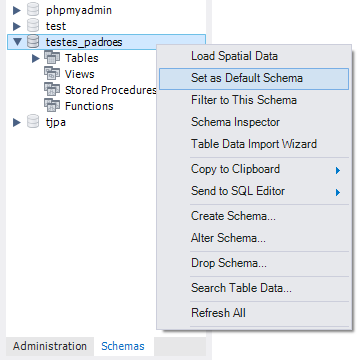
\includegraphics[scale=0.8]{imagens/cap04SelecionandoEsquema}
    \\\textbf{Fonte:} Elaborada pelo autor
    \label{fig:cap04SelecionandoEsquema}
\end{figure}
\FloatBarrier

Com a base ``testes\_padroes'' configurada como padrão, expanda-a e em \destaque{\textit{Tables}} clique com o botão direito e escolha \destaque{\textit{Create Table...}}. Vamos criar agora uma tabela que vai armazenar os dados de teste que iremos mexer durante este Capítulo. Preencha \destaque{\textit{Table Name:}} com ``pais'' (sem as aspas). \textit{Pais} é país, mas vamos omitir o acento tudo bem? Deixe os valores padrão nos campos \destaque{\textit{Charset/Collation:}}, \destaque{\textit{Engine:}} e \destaque{\textit{Comments:}}. Logo abaixo, clique duas vezes na primeira linha da coluna \destaque{\textit{Column Name}}. A ferramenta vai preencher o nome da primeira coluna automaticamente com o valor ``idpais''. Edite esse nome e deixe apenas ``id''. O tipo (Datatype) deve ficar como INT (inteiro) e as colunas \texttt{PK} (\textit{primary key}/chave primária), \texttt{NN} (\textit{not null}/não nulo) e \texttt{AI} (auto-increment/auto-incremento) devem ficar marcadas. Essa coluna da tabela será nossa chave primária. Agora vamos às outras colunas. Nossos países terão um nome e uma sigla. Então precisamos criar mais duas colunas, uma com nome de ``nome'' e a outra com nome de ``sigla''. A coluna ``nome'' terá o tipo \texttt{VARCHAR(100)}, ou seja, um \texttt{VARCHAR} de 100 posições e a coluna ``sigla'' terá o tipo \texttt{VARCHAR(2}). Marque essas duas colunas como \texttt{NN}, ou seja, elas terão dados obrigatoriamente quando um país for ser inserido na tabela. Veja como ficou na Figura~\ref{fig:cap04CriandoTabelaPais}.

\FloatBarrier
\begin{figure}[!htbp]
    \centering
    \caption{Criando a tabela ``pais''}
    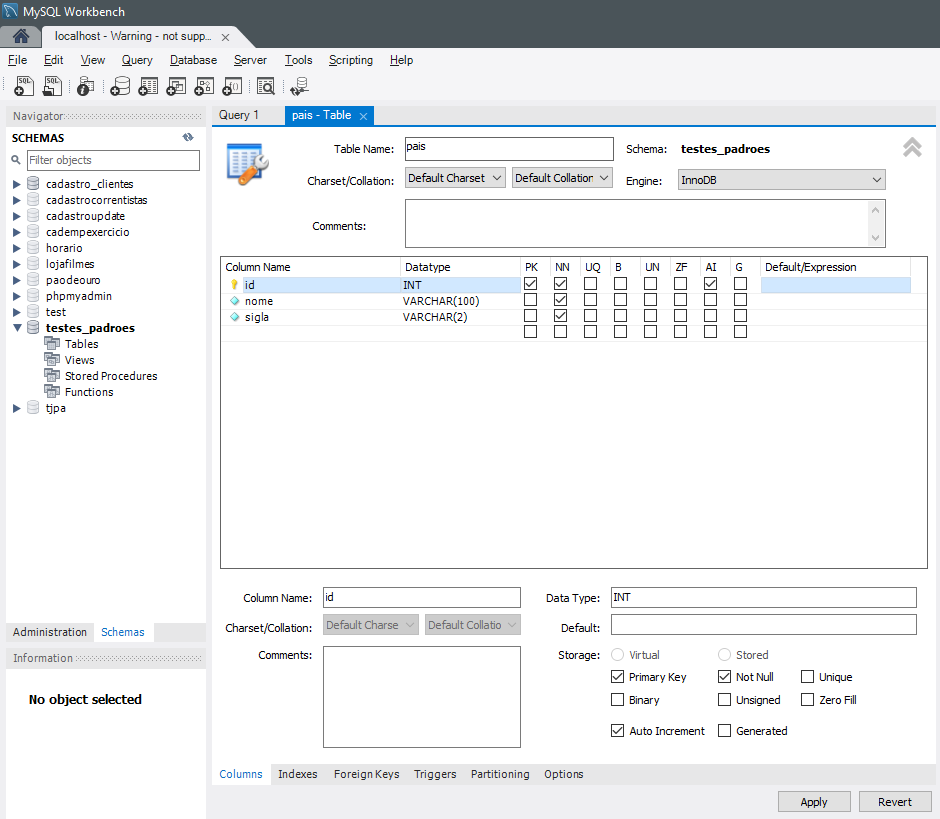
\includegraphics[scale=0.6]{imagens/cap04CriandoTabelaPais}
    \\\textbf{Fonte:} Elaborada pelo autor
    \label{fig:cap04CriandoTabelaPais}
\end{figure}
\FloatBarrier

Feito isso, clique em \destaque{\textit{Apply}}. Um diálogo será aberto para exibir o código SQL que será executado (Listagem~\thechapter.\ref{listagem:projetos/capitulo04/tabelaPais.sql}). Clique em \destaque{\textit{Apply}} e depois em \destaque{\textit{Finish}}. Pronto, criamos a nossa tabela para armazenar dados dos países, ela poderá ser vista do lado esquerdo, na aba \destaque{\textit{Schemas}}, dentro da base ``testes\_padroes''. Deixe o Workbench aberto e abra o NetBeans. 

\sqlCode{Instrução \texttt{CREATE TABLE} para a tabela ``pais''}{projetos/capitulo04/tabelaPais.sql}

\section{Padrão de Projeto Factory}

Primeiramente, vamos criar um novo projeto no NetBeans, só que agora ele não será um projeto Web, pois o que vamos fazer não precisa ser em um projeto desse tipo. Siga os passos que você está acostumado a fazer ao criar um projeto Java Web, só que desta vez escolha \destaque{\textit{Java with Ant}} na categoria e \destaque{\textit{Java Application}} nos tipos de projeto. Dê o nome de ``PadroesEmPratica'' para o projeto. Não se esqueça de marcar a opção \destaque{\textit{Use Dedicated Folder for Storing Libraries}}.

Como iremos conectar no banco de dados MariaDB, precisamos adicionar no nosso projeto a biblioteca que implementa esse conector. Infelizmente o NetBeans não vem com essa biblioteca pronta para ser usada, então teremos que baixá-la e inseri-la no projeto. Para isso, primeiro baixe o arquivo \texttt{.jar} da bibliteca no endereço \url{NOME}. Com o arquivo baixado, clique com o botão direito no nó \destaque{\textit{Libraries}} e escolha a opção \destaque{\textit{Add Library...}}. No diálogo que foi aberto, clique em \destaque{\textit{Create...}}. No diálogo que vai se abrir, preencha \destaque{\textit{Library Name:}} com ``MariaDB-ConnectorJ-2.7.3'' (ou o nome que você quiser) e em \destaque{\textit{Library Type}} deixe ``Class Libraries'' e clique em \destaque{\textit{OK}}. Mais um diálogo será aberto. Clique no botão \destaque{\textit{Add JAR/Folder...}} e procure pelo arquivo \texttt{.jar} da biblioteca que acabou de baixar. Selecione-se o clique em \destaque{\textit{Add JAR/Folder}}. Ao clicar nesse botão, um alerta perguntará se você que criar um diretório na pasta de bibliotecas do projeto, clique em \destaque{\textit{Yes}}. Agora clique no botão \destaque{\textit{OK}} do diálogo \destaque{\textit{Customize Library}} e, agora que a biblioteca foi criada, selecione-a no diálogo \destaque{\textit{Add Library}} e clique no botão \destaque{\textit{Add Library}}. Perceba que ao fazer isso, um aparecerá um novo nó dentro da pasta \destaque{\textit{Libraries}} do projeto com o nome da bibliteca que foi criada e adicionada.

A partir de agora, podemos conectar ao banco de dados a partir do nosso código. Como você deve saber, para que possamos usar um banco de dados em Java, nós usamos uma especificação chamada \textit{Java Database Connectivity} (JDBC). Essa especificação deve ser implementada pelos fabricantes dos Sistemas Gerenciadores de Bando de Dados (SGBD), permitindo assim que os programas feitos em Java possam se comunicar com estes SGBDs. Normalmente, esses pacotes que implementam o JDBC são chamados de ``Drivers JDBC'' e são obtidos nos sites dos fabricantes dos SGBDs.

A questão agora é: ``Como conectar no banco de dados?''. Para que possamos conectar no MariaDB, existem uma série de ``comandos'' que precisamos fazer cada vez que queremos estabelecer uma conexão. Você, como desenvolvedor, sabe que uma boa prática de programação é encapsular trechos de código que fazem uma determinada tarefa em funções e que as funções em Java são chamadas de métodos.

Legal, mas e o que o tal do ``padrão de projeto'' tem haver com isso? Ou melhor, o que é um padrão de projeto? O termo padrão de projeto (\textit{design pattern} em inglês) foi criado por Christopher Alexander \cite{Alexander1977} na década de 1970 para designar soluções de sucesso para problemas recorrentes na área da arquitetura. Alexander definiu nessa época uma série de padrões que apresentavam soluções padrão para problemas que aconteciam de forma corriqueira, sendo que uma série de padrões correlatos foram o que podemos chamar de linguagem de padrões. A partir do termo cunhado por Alexander, alguns programadores começaram a criar padrões de projeto para a computação, iniciando esse trabalho do domínio da programação orientada a objetos.

O livro ``Padrões de Projeto: Soluções Reutilizáveis de Software Orientado a Objetos'' \cite{Gamma2000} é a referência básica para os padrões de projeto criados para resolver problemas relacionados ao desenvolvimento orientado a objetos. A partir de agora, quando você ler ``padrão de projeto'', entenda que estarei falando de padrões relacionados ao desenvolvimento de software orientado a objetos, tudo bem? Sendo assim, o primeiro padrão que iremos aprender se chama \textit{Factory} (fábrica). 

Vamos entender o contexto do padrão. Imagine que no seu programa você precisa criar e utilizar um determinado tipo de objeto muitas e muitas vezes e que este objeto precisa ser inicializado com uma série de valores, sendo que esses valores normalmente são sempre os mesmos. Assim, cada vez que você instância esse objeto, você precisa executar uma determinada quantidade de código. Como resolver isso? Criar um método que faça essa tarefa é uma boa solução não é mesmo? Mas em qual classe eu vou escrever esse método? No padrão \textit{Factory}, nós criamos classes especializadas que serão fábricas de objetos e que terão um método que executará a tarefa da fábrica, ou seja, criar um determinado tipo de objeto.

No nosso projeto, um tipo de objeto que usaremos muito, é um objeto que representa a conexão entre nosso programa escrito em Java e o SGBD. Sendo assim, nós precisamos de uma fábrica de conexões! Vamos implementar a fábrica? No projeto que você criou agora a pouco, o NetBeans gerou por padrão um pacote chamado ``padroesempratica'' dentro da pasta \destaque{\textit{Source Packages}}. Crie dentro deste pacote outro com o nome de ``jdbc'' (sem as aspas) e dentro do pacote ``padroesempratica.jdbc'', crie uma classe Java com o nome de ``ConnectionFactory'' (sem as aspas). Essa classe conterá o método que vai fabricar a conexão. Veja o código dela na ListagemListagem~\thechapter.\ref{listagem:projetos/capitulo04/PadroesEmPratica/src/padroesempratica/jdbc/ConnectionFactory.java}.

\javaCode{Uma fábrica de conexões (\texttt{padroesempratica/jdbc/ ConnectionFacotory.java})}{projetos/capitulo04/PadroesEmPratica/src/padroesempratica/jdbc/ConnectionFactory.java}

Copiou o código? Ótimo! Esta classe tem um método estático chamado \texttt{getConnection()} que vai fabricar a conexão para nós e que caso ocorra algum problema, vai lançar uma exceção do tipo SQLException. Toda vez que chamarmos esse método, ele vai retornar uma nova conexão para nós e o Driver JDBC apropriado será carregado automaticamente pelo \texttt{DriverManager}. 

Agora precisamos testar esse método para ver se não está havendo nenhum erro. Clique novamente com o botão direito no pacote ``padroesempratica'' e crie um novo pacote chamado ``testes''. Dentro do pacote ``padroesempratica.testes'', crie uma classe chamada ``TesteConnectionFactory''. Como você deve saber, para que uma classe em Java possa ser executada, nós precisamos implementar o método \texttt{main} com uma determinada assinatura. O que vamos fazer no método \texttt{main} da classe ``TesteConnectionFactory'' é tentar criar uma conexão e ver se nenhum erro é retornado. Na Listagem~\thechapter.\ref{listagem:projetos/capitulo04/PadroesEmPratica/src/padroesempratica/testes/TesteConnectionFactory.java} você pode ver o código desta classe.

\javaCode{Classe para teste de conexão (\texttt{padroesempratica/testes/ TesteConnectionFactory.java})}{projetos/capitulo04/PadroesEmPratica/src/padroesempratica/testes/TesteConnectionFactory.java}

Copie o código para a classe e salve o arquivo. Para executarmos apenas uma classe que tem o método \texttt{main}, basta clicar com o botão direito no editor e escolhe a opção \destaque{\textit{Run File}}, ou então, com o arquivo aberto no editor, usar o atalho \texttt{<Shift+F6>}. Fazendo isso, a classe vai ser compilada e executada pelo NetBeans. Se tudo estiver correto, você verá na saída a mensagem ``Conexão criada com sucesso!''. Deu erro? Verifique se o código da classe \texttt{ConnectionFactory} está correto e se a senha do usuário \texttt{root}, definida dentro do método \texttt{getConnection} está correta. No nosso caso, ela é vazia. Agora que está tudo certo, vamos simular um erro. Entre na classe \texttt{ConnectionFactory} e coloque uma senha inválida (terceiro parâmetro do método \texttt{getConnection} de \texttt{DriverManagaer}) para o usuário \texttt{root}, por exemplo, ``123''. Volte na classe de testes e execute-a novamente (\texttt{<Shift+F6>}). Gerou um erro não foi? A mensagem ``Erro ao tentar criar a conexão!'' deve ter sido exibida, seguida de várias linhas que explicam o erro ocorrido. A primeira linha dos erros diz que o acesso foi negado para o usuário ``root@localhost'' não foi? Por que aconteceu isso? Porque a senha está errada! Volte na fábrica de conexões e coloque a senha correta (vazia). Teste novamente. Agora deve estar tudo certo.

Legal, temos uma fábrica de conexões, mas do que adianta uma fábrica de alguma coisa se a gente não usar o que é fabricado? Vamos para o próximo padrão, onde iremos organizar uma camada de persistência para nossa aplicação e usaremos a fábrica de conexões para viabilizar a comunicação entre nossa aplicação e o SGBD.


\section{Padrão de Projeto \textit{Data Access Object} (DAO)}

Quando temos o nosso primeiro contato com JDBC, normalmente nos é ensinado a colocar todo o código SQL que vai executar uma determinada operação em um método que trata o ``clique'' de um botão. Sendo assim, imagine uma interface desktop (em Swing) onde poderíamos criar, alterar e/ou excluir países. Quando implementamos o botão responsável por criar um novo país, somos ensinados a inserir todo o código SQL para fazer isso, sendo que esse código é implementado usando uma cláusula INSERT. O mesmo aconteceria para os botões alterar e excluir. Será que essa é a melhor solução? Será que a classe que implementa nossa interface gráfica tem que ter essa responsabilidade, ou seja, lidar com SQL? E se por algum motivo nós quiséssemos usar o código para criar um novo país em alguma outra tela? Teríamos que copiar o código de inserção novamente? Tenho certeza que para essa última pergunta você já deve ter respondido mentalmente que ``NÃO!'', pois podemos criar métodos que executariam essa operação, mas então te pergunto: Como fazer isso?

Para resolver esse problema, existe um padrão de projeto onde a ideia é isolar todo acesso ao banco de dados em classes que seriam responsáveis em fazer a comunicação entre a aplicação Java, ou qualquer aplicação escrita usando uma linguagem orientada a objetos, e o banco de dados. Esse padrão se chama DAO (Data Access Object – Objeto de Acesso a Dados), sendo este um dos mais famosos. Vamos aprender como implementá-lo?

Um objeto do tipo DAO deve ter a capacidade de executar as operações básicas sobre uma determinada tabela de um banco de dados. Essas operações são comumente chamadas de CRUD (Create, Read, Update e Delete – Criar, Ler, Atualizar e Excluir). Praticamente cada tabela do nosso banco de dados terá no lado da aplicação uma classe implementada que representa um registro da tabela (tabela ``pais'', classe Pais), além de ter uma classe DAO que vai manipular objetos do tipo Pais. Como precisamos definir essas quatro operações básicas que cada DAO vai conter, vamos criar uma classe abstrata que servirá de modelo.

No pacote ``padroesempratica'', crie um novo pacote chamado ``dao''. Dentro do pacote ``padroesempratica.dao'', crie uma classe chamada ``DAO'' e copie o código apresentado na Listagem 4.3 e na Listagem 4.4. Note que as duas listagens são partes da mesma classe.


Listagem~\thechapter.\ref{listagem:projetos/capitulo04/PadroesEmPratica/src/padroesempratica/dao/DAO.java}
\javaCode{Implementação da classe abstrata DAO (\texttt{padroesempratica/dao/DAO.java})}{projetos/capitulo04/PadroesEmPratica/src/padroesempratica/dao/DAO.java}


Copiou o código? Ótimo! Vamos entendê-lo. Na linha 13 da Listagem 4.3 definimos uma classe abstrata (classes abstratas não podem ser instanciadas, são usadas como modelos) chamada DAO que diz que toda classe que for implementá-la, deve definir um tipo ``T'' que obrigatoriamente estende Object. As construções entre ``<'' e ``>'' são chamadas de ``Tipos Genéricos'' em Java. Note que o tipo ``T'' é usado em todo o corpo da classe. Está confuso? Acalme-se, logo você vai entender.

Na linha 16 da Listagem 4.3 é declarada uma conexão, que sempre será obtida usando o método getConnection definido na linha 39. Observe que poderíamos ter declarado essa conexão como protected, mas vamos deixá-la como private e usar o método getConnection() para obtê-la. Na linha 49 é definido o método para fechar a conexão, afinal, sempre que usarmos uma conexão, precisamos fechá-la depois de usar.

Veja que no construtor da classe (linha 24 da Listagem 4.3), a conexão é obtida usando a fábrica que criamos na seção anterior! Esse construtor será executado quando instanciarmos os objetos das classes que estenderem esse DAO, então, quando criarmos nossos objetos DAO, uma conexão com o banco de dados será estabelecida.

A partir da linha 60 da Listagem 4.4 são definidos todos os métodos CRUD deste DAO genérico. Note que temos dois métodos que correspondem à parte ``R'' do CRUD, onde um obtém todas as entidades cadastradas e outro obtém apenas uma usando como base seu identificador.

Com o DAO genérico pronto, vamos implementar a classe que vai representar a tabela ``pais''. Crie um novo pacote chamado ``entidades'' dentro do pacote ``padroesempratica''. Dentro do pacote ``padroesempratica.entidades'', crie uma classe chamada ``Pais'' (sem as aspas). Os objetos dessa classe representarão registros da tabela ``pais'', sendo assim, precisamos que essa classe tenha os mesmos atributos da tabela correspondente. Lembre-se que na tabela ``pais'' nós definimos três colunas: id (INT), nome (VARCHAR) e sigla (VARCHAR). Na nossa classe, iremos usar o tipo ``int'' como tipo correspondente ao INT da tabela. Para o tipo VARCHAR, usaremos Strings. Veja na Listagem 4.5 como deve ficar a implementação parcial da classe Pais.

Listagem~\thechapter.\ref{listagem:projetos/capitulo04/parciais/Pais.java}
\javaCode{Implementação parcial da classe Pais (\texttt{padroesempratica/entidades/Pais.java})}{projetos/capitulo04/parciais/Pais.java}

Tenho certeza que você se lembra da discussão sobre o padrão JavaBeans não é mesmo? Onde foi dito que devemos expor ao mundo ``fora da classe'' os atributos que nós queremos que possam ser configurados e obtidos por seus utilizadores? Da primeira vez que falamos sobre isso, nós implementamos manualmente cada método set e get correspondente a um campo privado não foi? Como essa tarefa é muito corriqueira, o NetBeans tem uma funcionalidade que faz isso automaticamente para nós. Com a classe implementada, como exibido na Listagem 4.5, clique com o botão direito no editor e escolha ``Inserir código...''. Veja na Figura 4.4.

Figura 4.4: Usando o assistente de inserção de código
 
Fonte: Print screen, NetBeans IDE 6.9.1

Ao clicar nesta opção, uma pequena lista com o nome de ``Gerar'' será exibida no editor. Nessa lista, escolha a opção ``Getter e setter...''. Adivinhe o que vamos fazer? Gerar os métodos get e set para cada campo da classe! Fazendo isso, um diálogo será exibido, mostrando todos os campos privados da classe. Marque cada um dos campos clicando na caixa de seleção correspondente, ou então, a classe inteira e clique no botão ``Gerar''. Veja o que aconteceu! A ferramenta gerou o código dos gets e sets para nós! Segue na Listagem 4.6 o código completo da classe Pais.

Listagem~\thechapter.\ref{listagem:projetos/capitulo04/PadroesEmPratica/src/padroesempratica/entidades/Pais.java}
\javaCode{Implementação da classe Pais (\texttt{padroesempratica/ entidades/Pais.java})}{projetos/capitulo04/PadroesEmPratica/src/padroesempratica/entidades/Pais.java}

Muito legal não é mesmo? Agora que temos a classe que representa a estrutura da tabela ``pais'' da nossa base de dados, vamos implementar nosso primeiro DAO concreto, ou seja, uma classe que vai estender a classe abstrata DAO. Novamente, no pacote ``padroesempratica.dao'', crie uma classe chamada ``PaisDAO'' (sem as aspas). Essa classe irá lidar com os objetos do tipo Pais, fazendo a ponte entre nossos objetos e o banco de dados. Com a classe criada, copie o código apresentado na Listagem 4.7.

Listagem~\thechapter.\ref{listagem:projetos/capitulo04/parciais/PaisDAOP1.java}
\javaCode{Implementação parcial da classe PaisDAO (\texttt{padroesempratica/ dao/PaisDAO.java})}{projetos/capitulo04/parciais/PaisDAOP1.java}

Veja que nosso PaisDAO vai estender DAO, informando como tipo a classe Pais (DAO<Pais>). Ao copiar o código, você perceberá que o NetBeans vai reclamar, dizendo que tem um erro na classe. O nome da classe ficará destacado em vermelho. Passe o mouse por cima do nome e aguarde. Será exibida a causa do erro. No erro, é dito que a classe PaisDAO não implementa todos os métodos abstratos da classe DAO e isso é verdade, visto que como estamos estendendo a classe DAO, precisamos implementar todos os métodos abstratos que foram definidos nela e ainda não fizemos isso. Teríamos então que implementar manualmente todos os métodos marcados como abstratos na classe DAO. Ao invés de fazermos isso manualmente, o NetBeans pode nos ajudar novamente. Veja que na linha do erro, à esquerda, é mostrada uma pequena lâmpada. Clique nela. Ao clicar, o NetBeans vai listar as alternativas que ele pode executar para resolver o erro. No caso, apenas uma opção será listada (``Implementar todos os métodos abstratos'') veja a Figura 4.5.

Figura 4.5: Implementando automaticamente os métodos abstratos de DAO
 
Fonte: Print screen, NetBeans IDE 6.9.1

Clique nesta opção e, novamente, como num passe de mágica, o NetBeans gera todo o esqueleto da classe para nós, criando uma implementação padrão para cada método abstrato da classe DAO. Mesmo ao fazer isso, o NetBeans continua reclamando que existe um erro. Nesse caso, é dito que é lançada uma exceção no construtor padrão. Você se lembra que lá no DAO genérico nós temos um construtor que cria a conexão e que ele lança uma SQLException? Pois bem, quando criamos um objeto de uma determinada classe, o construtor da superclasse da classe em questão é executado. Como estendemos DAO em PaisDAO, ao tentarmos instanciar um objeto do tipo PaisDAO, o construtor de PaisDAO será executado, além do construtor de DAO, que é sua superclasse. Como o construtor de DAO lança uma exceção caso ocorra algum problema, nós precisamos ou tratar ou dizer que o construtor de PaisDAO também lança esse tipo de exceção. Nós iremos usar a segunda abordagem. Para isso, basta implementar o construtor padrão de PaisDAO e dizer que ele lança esse tipo de exceção. Sendo assim, segue na Listagem 4.8 a implementação que temos até agora da classe PaisDAO.

<Glossário: Construtor Padrão
O construtor padrão é o construtor que não tem nenhum parâmetro.
>

Listagem~\thechapter.\ref{listagem:projetos/capitulo04/parciais/PaisDAOP2.java}
\javaCode{Implementação parcial da classe PaisDAO com o construtor padrão (\texttt{padroesempratica/ dao/PaisDAO.java})}{projetos/capitulo04/parciais/PaisDAOP2.java}

Muito bom. Até agora preparamos toda o esqueleto do nosso PaisDAO, mas SQL que é bom, nada. Vamos agora implementar nosso primeiro método do CRUD, o ``salvar''. Para poupar espaço, irei listar apenar o método em questão, ao invés de listar a classe completa, tudo bem? Lembre-se que estamos implementando o método ``salvar'' da classe PaisDAO. Antes de implementar o método ``salvar'', importe a classe ``java.sql.PreparedStatement''. Na Listagem 4.9 pode ser vista a implementação do método ``salvar'' da classe PaisDAO.

Listagem~\thechapter.\ref{listagem:projetos/capitulo04/parciais/PaisDAOSalvar.java}
\javaCode{Implementação do método ``salvar'' da classe PaisDAO (\texttt{padroesempratica/ dao/PaisDAO.java})}{projetos/capitulo04/parciais/PaisDAOSalvar.java}

Vamos analisar o código para ver o que está acontecendo. Na linha 2 está definida a assinatura do método. O método ``salvar'' recebe um parâmetro do tipo Pais, sendo que os dados do objeto passado nesse parâmetro serão persistidos no banco de dados. Nas linhas 4 e 5 é definida a cláusula INSERT do banco de dados. Como a coluna id de pais foi definida como auto incremento, nós não precisamos fornecê-la. Ao invés de definirmos manualmente os valores das colunas nome e sigla, perceba que utilizamos sinais de interrogação, indicando que no lugar de cada ponto de interrogação será trocado pelo valor correto. Na linha 7 é criado um PreparedStatement a partir da conexão do DAO usando o código SQL que foi definido nas linhas 4 e 5. Na linha 8, o primeiro parâmetro do código SQL (primeiro ponto de interrogação) é trocado pelo valor retornado pelo método getNome() do objeto ``obj'' do tipo Pais. A mesma coisa acontece na linha 9, onde o segundo parâmetro do código SQL (segundo ponto de interrogação) é trocado pelo valor retornado pelo método getSigla(). Com o PreparedStatement configurado, na linha 11 mandamos que seja executado o PreparedStatement. Por fim, na linha 12, fechamos o PreparedStatement. Fácil não é?

Vamos testar? No pacote ``padroesempratica.testes'', crie uma classe chamada TestePaisDAO e copie o código da Listagem 4.10.

Listagem~\thechapter.\ref{listagem:projetos/capitulo04/PadroesEmPratica/src/padroesempratica/testes/TestePaisDAO.java}
\javaCode{Código de teste para o PaisDAO (\texttt{padroesempratica/ testes/TestePaisDAO.java})}{projetos/capitulo04/PadroesEmPratica/src/padroesempratica/testes/TestePaisDAO.java}

Copiou o código? Execute a classe (botão direito no arquivo, ``Executar arquivo'' ou Shift+F6). Se tudo estiver correto, a classe será compilada e executada e nenhum erro será emitido. Fazendo isso, um novo registro na tabela ``pais'' será gerado. Vamos confirmar isso? No MySQL Workbench, abra o editor de SQL clicando duas vezes na conexão definida na seção ``SQL Development''. Provavelmente o editor já deve estar aberto. Em ``Object Browser'' selecione a base ``testes\_padroes'' em ``Default''. Em ``Scratch'', entre digite ``select * from pais;'' (sem as aspas) e clique no botão que tem um desenho de um raio na barra de tarefas. O código SQL digitado será executado e o resultado será exibido logo abaixo. Veja a Figura 4.6.

Figura 4.6: Fazendo uma consulta do MySQL Workbench
 
Fonte: Print screen, MySQL Workbench

Muito bem! Nosso método salvar está funcionando corretamente. Vamos analisar o código da Listagem 4.10. Entre as linhas 16 e 18 instanciamos e configuramos um objeto do tipo Pais. O nome desse país é Brasil e a sigla é BR. Na linha 20, declaramos uma referência do tipo PaisDAO que foi inicializada com null. Como todo o código dos métodos do DAO podem lançar uma exceção do tipo SQLException, temos que usar um bloco try. Na linha 24 instanciamos o PaisDAO e na linha 25 passamos o objeto do tipo Pais que criamos para o método ``salvar'' do DAO, que por sua vez vai executar o código SQL que definimos. Caso ocorra algum problema durante a execução de uma dessas duas linhas, o catch que ouve exceções do tipo SQLException captura o erro e manda mostrar esses problemas dando um printStackTrace() no objeto que representa a exceção. Por fim, temos um bloco finally que trata do fechamento da conexão. Sempre quando usarmos um DAO, precisamos fechar sua conexão quando terminarmos de usar. Na linha 33 verifica-se se o ``dão'' aponta para null. Se não apontar, tenta fechar a conexão, que também pode lançar uma exceção do tipo SQLException e que é tratada dentro do bloco try que está aninhado no finally.

Agora que já criamos e testamos nosso primeiro método do PaisDAO, vamos implementar o restante dos métodos. Cada um deles será apresentado em uma listagem diferente. Os métodos de pesquisa (``R'' do CRUD) serão um pouco diferente, sendo assim, eu os discutirei depois. Vamos lá!

Listagem~\thechapter.\ref{listagem:projetos/capitulo04/PadroesEmPratica/src/padroesempratica/dao/PaisDAO.java}
\javaCode{Implementação da classe PaisDAO (\texttt{padroesempratica/ dao/PaisDAO.java})}{projetos/capitulo04/PadroesEmPratica/src/padroesempratica/dao/PaisDAO.java}

Não se esqueça de importar as classes java.sql.ResultSet, java.util.ArrayList e import java.util.List. Para finalizar essa seção, vamos discutir o código da Listagem 4.13. O método listarTodos retorna uma lista que pode conter apenar objetos do tipo Pais. Essa lista que será retornada é instanciada e inicializada na linha 4. Neste momento, temos a lista de objetos do tipo Pais, só que ela ainda está vazia. Na linha 7, cria-se o PreparedStatement com o SQL que foi definido na linha 5 e, na linha 8, executamos o PreparedStatement usando o método executeQuery(), que retorna um objeto do tipo ResultSet. Os objetos do tipo ResultSet representam os resultados que são retornados em consultas SQL (comando SELECT). Na linha 10, criamos um laço de repetição while, que é executado enquanto rs.next() retornar true. Na primeira vez que rs.next() é invocado, o ponteiro de registros do ResultSet passa a apontar para o primeiro resultado obtido na consulta. Dentro do while, entre as linhas 12 e 15, nós criamos um objeto do tipo Pais e configuramos seus dados a partir dos dados obtidos no ResultSet, usando o método apropriado para cada tipo de cada coluna. Na linha 17, o objeto Pais que acabou de ser criado e configurado, é inserido na lista. O corpo do while é repetido até que rs.next() retorne false, ou seja, quando todos os resultados da consulta foram obtidos. Nesse ponto, temos a lista de objetos totalmente preenchida. Nas linhas 21 e 22, são fechados o ResultSet e o PreparedStatement. Por fim, na linha 24, a lista com os objetos do tipo Pais é retornada.

Note que o método ``obterPorId'', definido na Listagem 4.14, tem uma implementação muito parecida com o método ``listarTodos'', só que no caso do ``obterPorId'', apenas um objeto pode ser retornado, visto que cada registro da tabela pais tem um identificador específico. Caso o id passado como parâmetro não represente um registro da tabela pais, o método retorna null.

Agora, como exercício, modifique a classe TestePaisDAO para testar todos os métodos que foram implementados. Verifique se todos estão corretos usando o MySQL Workbench para comparar os resultados obtidos. Tente entender a implementação de cada método do CRUD.

Não fez o exercício? Então faça! Ele não é opcional.

Viu só que legal? Com tudo isso que fizemos, conseguimos isolar toda a camada de persistência da nossa aplicação. Para cada tabela nova que tivermos na base de dados, precisamos implementar a classe correspondente à tabela (que chamamos de entidade) e a classe DAO que vai manipular os objetos da classe criada e fazer o intercâmbio entre o mundo orientado a objetos com o mundo relacional. Essa comunicação entre objetos e o modelo relacional, é chamada de ORM (Object-Relational Mapping – Mapeamento Objeto-Relacional). Existem diversos frameworks que automatizam esse processo, gerando todo o código SQL automaticamente para nós. Infelizmente não teremos tempo para aprendê-los. Um desses frameworks é o Hibernate.

<Saiba mais:
Quer saber mais sobre ORM? Acesse os links a seguir:
http://pt.wikipedia.org/wiki/Mapeamento\_objeto-relacional
http://en.wikipedia.org/wiki/Object-relational\_mapping (em inglês)
http://www.hibernate.org/
>
Estamos quase acabando! Vamos para o último padrão de projeto.



\section{Padrão de Projeto \textit{Model-View-Controller} (MVC)}


O padrão MVC (Model-View-Controller – Modelo-Visualização-Controle) é um padrão muito utilizado no desenvolvimento de aplicações que utilizam linguagens orientadas a objetos. Este padrão ajuda os desenvolvedores a separar as regras de negócio da aplicação, ou seja, as regras de como os dados devem se armazenados, qual a ordem que devem ser gravados, etc., da lógica de apresentação desses dados, ou seja, como eles serão exibidos aos usuários do sistema. Essa separação se dá utilizando três camadas: 

•	Model (Modelo): A camada Model é usada para organizar como a informação é armazenada e gerenciada dentro da aplicação. No exemplo que construímos durante esta aula, as classes Pais e PaisDAO fazem parte do modelo.

•	View (Visualização): Essa camada organiza os recursos utilizados para exibir ao usuário os dados que são gerenciados pela camada de modelo.

•	Controller (Controle): A camada Controller, como o próprio nome já diz, é responsável por controlar o fluxo de execução da aplicação.

A partir dessas definições, nós podemos ver nitidamente, nos exemplos que estamos construindo desde o início da disciplina, qual recurso faz parte de cada camada. A entidade Pais faz parte do modelo. Uma JSP faz parte da visualização, pois é usada pelo usuário tanto para inserir dados no sistema quanto para visualizá-los. Os Servlets que construímos fazem parte do controle, pois são eles que recebem os dados, os utilizam usando a camada de modelo e decidem para onde o fluxo da aplicação deve ser direcionado, por exemplo, uma página JSP que vai exibir a saída gerada por eles.

Essa foi uma pequena introdução do MVC, pois durante a próxima aula nós iremos usá-lo extensivamente no projeto que iremos criar. Tenho certeza que você vai achar muito legal e útil! Como de costume, pratique o que você aprendeu durante esta aula, com as atividades de aprendizagem.



\section{Resumo}

Nesta aula demos um passo muito importante na nossa vida como desenvolvedores. Nós aprendemos que existem os chamados ``padrões de projeto'' ou ``design patterns'', que são padrões que guiam os desenvolvedores na solução de problemas recorrentes através do uso de soluções de sucesso. Estudamos os padrões Factory e DAO implementando exemplos e aprendemos o básico do funcionamento do padrão MVC. Na próxima aula iremos implementar um projeto completo usando esses três padrões. 


\section{Exercícios}

1 – Defina, com suas palavras, o padrão Factory.
2 – Defina, com suas palavras, o padrão DAO.
3 – Defina, com suas palavras, o padrão MVC.
4 – Da mesma forma que fizemos para a tabela ``pais'', crie uma tabela no MySQL, usando o Workbench, com o nome de ``fruta''. Essa tabela deve ter como colunas um campo identificador (id), um campo que armazenará o nome da fruta (VARCHAR) e um campo para armazenar a cor predominante da fruta (VARCHAR). Implemente, no projeto que criamos durante a Aula 4, a entidade Fruta e a classe FrutaDAO. Crie uma classe de testes chamada TesteFrutaDAO para testar os métodos do DAO da fruta. 
5 – Repita a atividade 4, só que agora para a tabela ``carro''. Um carro deve ter um identificador, um nome (VARCHAR), um modelo (VARCHAR) e um ano de fabricação (INT).
6 – Repita a atividade 4, só que agora para a tabela ``produto''. Um produto deve ter um identificador, uma descrição (VARCHAR) e uma quantidade em estoque (INT).


\section{Projetos}